\documentclass[]{article}

\usepackage{enumerate}
\usepackage{amssymb}
\usepackage{graphicx}

\def\OR{\vee}
\def\AND{\wedge}
\def\imp{\rightarrow}
\def\math#1{$#1$}
\def\mand#1{$$#1$$}
\def\mld#1{\begin{equation}
#1
\end{equation}}
\def\eqar#1{\begin{eqnarray}
#1
\end{eqnarray}}
\def\eqan#1{\begin{eqnarray*}
#1
\end{eqnarray*}}
\def\cl#1{{\cal #1}}

\DeclareSymbolFont{AMSb}{U}{msb}{m}{n}
\DeclareMathSymbol{\N}{\mathbin}{AMSb}{"4E}
\DeclareMathSymbol{\Z}{\mathbin}{AMSb}{"5A}
\DeclareMathSymbol{\R}{\mathbin}{AMSb}{"52}
\DeclareMathSymbol{\Q}{\mathbin}{AMSb}{"51}
\DeclareMathSymbol{\I}{\mathbin}{AMSb}{"49}
\DeclareMathSymbol{\C}{\mathbin}{AMSb}{"43}

\begin{document}
\bf \Large Gabriel Maayan - FOCS Assignment 3

\section{DMC 5.4}
Only (ii) is a valid way of proving \math{F(n)=P(n)\to P(n+1)}
because when proving \math{P\to Q}, proving \math{Q=f\to P=f} 
is the only way to prove \math{F(n) = t}


\section{DMC 5.3}
\begin{enumerate}[(c)]
\item \math{P(n)\to P(n^2)\land P(n-2)
\\ P(2)\to P(4)\land P(0)
\\ P(4)\to P(16)\land P(2)
\\ P(16)\to P(256)\land P(14)
\\ \vdots
\\} \math{P} is true for \math{n=2k, k\in \Z}

\end{enumerate}
\section{5.11}
\begin{enumerate}[(b)]
\item For \math{0\leq x\leq \frac{1}{2}}, \math{-2x\leq ln(1-x)\leq -x
\\ x=\frac{1}{n+1}
\\ \frac{-2}{n+1}\leq ln(\frac{n}{n+1})\leq \frac{-1}{n+1}
\\ \frac{-2}{n+1}\leq ln(n)-ln(n+1)\leq \frac{-1}{n+1}
\\ \therefore} (a) \math{ ln(n+1) - \frac{2}{n+1} \leq ln(n)} and (b) \math{ln(n)\leq ln(n+1)-\frac{1}{n+1}
\\ \\ P(n) : 1+\frac{1}{2}ln(n) \leq H_n \leq 1+ln(n)
\\ P(n+1) : 1+\frac{1}{2}ln(n+1) \leq H_{n+1} \leq 1+ln(n+1)
\\ \\} By (a) : \math{1+\frac{1}{2}(ln(n+1)-\frac{2}{n+1})\leq H_n
\\ 1+\frac{1}{2}ln(n+1)-\frac{1}{n+1}\leq H_n
\\ 1+\frac{1}{2}ln(n+1)\leq H_{n+1}
\\ \\} By (b) : \math{ln(n)\leq ln(n+1) -\frac{1}{1+n}
\\ H_n\leq 1+ln(n+1)-\frac{1}{n+1}
\\ H_{n+1}\leq 1+ln(n+1)
\\ \therefore 1+\frac{1}{2}ln(n) \leq H_n \leq 1+ln(n)}


\end{enumerate}
\section{DMC 5.43}
\begin{enumerate}[(a)]
\item The robot is at position (3, 3), it wants to get to position (3, 4)
\math{\\} Let \math{n=x+y}, position \math{=(x, y)\\}
So the robot starts at a position of \math{n=6} and wants to get to
 a position of \math{n=7}. However, since it can only move diagonal, 
the only possible \math{\Delta n} is \math{\pm 0} or \math{\pm 2\\}
Therefore, it is only ever possible for the robot to move onto even n-numbered 
squares and thus can never reach (3, 4).

\item Following the same logic as above, the new possible \math{\Delta n}'s are 
\math{\pm 0, +3, -2}, so now the robot can reach odd n-numbered squares, 
as well as even n-numbered squares, and thus can reach all squares in a 
finite number of moves.

\end{enumerate}
\section{DMC Exercise 6.2}
Assume \math{P(n) : n^3 < 2^n, n\geq 10\\}
Prove \math{n^3+3n^2+3n+1 < 2^{n+1}\\
n^3 < 2^n
\\ 3n^2+3n+1 < n^3 < 2^n} for \math{n\geq 10\\
\therefore n^3+3n^2+3n+1 < 2^n + 3n^2 + 3n +1 < 2^n + 2^n
\\ \therefore (n+1)^3 < 2^{n+1}}

\section{DMC Exercise 6.4}
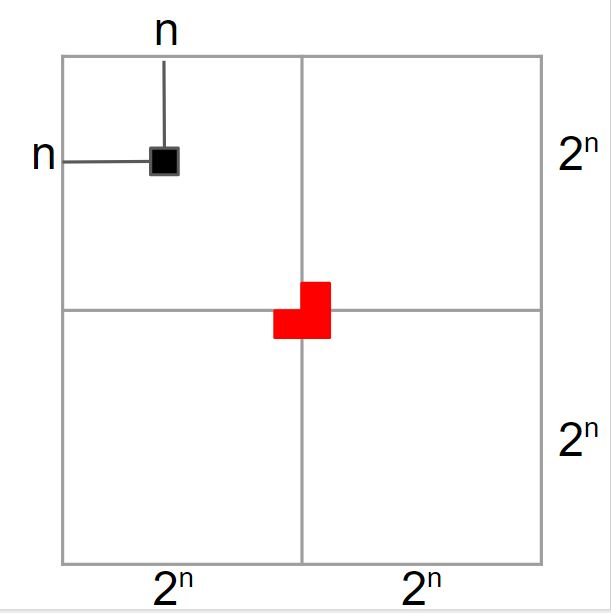
\includegraphics[width=\linewidth]{FOCSHW3}
Assume that if a missing square is at position \math{(n, n)} on a \math{2^n}x\math{2^n}
patio, you can still L-tile the patio.\math{\\}
A \math{2^{n+1}}x\math{2^{n+1}} patio with a missing square at \math{(n, n)}, with a 
tile placed in the center, as shown in the Figure above, can be broken up into 4 \math{2^n}x\math{2^n}
patios, 1 with a center tile missing and 3 with a corner tile missing. By the proof given 
in Chapter 6.1 : L-Tile Land of DMC, both of these types of \math{2^n}x\math{2^n} patios 
can be tiled individually, therefore the \math{2^{n+1}}x\math{2^{n+1}} patio can be tiled.

\end{document}
